\chapter{Didaktické príklady}
\label{Didaktické príklady}

Pre AeroShield bolo v prostredí Arduino IDE, MATLAB a Simulink vytvorených niekoľko vzorových programov, ktoré demonštrujú všetky jeho funkcie a možnosti operácie. Programy sú rozdelené do dvoch veľkých skupín, konkrétne programy v otvorenej slučke bez spätnej väzby a programy v uzavretej slučke so spätnou väzbou. 

Ich rozdiel spočíva v tom že pri riadení bez spätnej väzby, hovoríme o ovládaní systému, kedy sa snažíme dosiahnuť žiadané hodnoty výstupov bez spätnej informácie o vykonaní procesu, alebo o jeho hodnote. V prípade riadenia so spätnou väzbou sa jedná o reguláciu. Pri regulácii sa kontroluje bezprostredný účinok riadenia, ktorý sa porovnáva so žiadanou hodnotou výstupu a na vyrovnanie ich vzájomnej chyby, sa okamžite vykonáva zásah do vstupných veličín. 

\section{Programy v otvorenej slučke, bez spätnej väzby}
\subsection{Arduino IDE}

Ako prvý príklad si ukážeme program s názvom \verb|AeroShield_OpenLoop.ino| napísaný v prostredí Arduino IDE. Hlavnou ideou tohoto programu je jednoduché ovládanie otáčok motorčeka kyvadla, pomocou potenciometra. Na začiatku programu inicializujeme hlavnú knižnicu AeroShieldu pomocou príkazu \verb|#include "AeroShield.h"|. Následne deklarujeme premenné, ktorých hodnoty budú vypisované na sériový monitor. 

\begin{lstlisting}[caption={AeroShield open loop dekleracia.},captionpos=b]
#include "AeroShield.h"       //  Inicializacia hlavnej kniznice

float startangle=0;           //  Premenna pre nulovy uhol
float lastangle=0;            //  Premenna pre maximalny uhol 
float pendulumAngle;          //  Uhol natocenia kyvadla
float referencePercent;       //  Hodnota potenciometra
float CurrentMean;	      //  Hodnota prudu odoberaneho motorom 
\end{lstlisting}

Nasleduje časť \verb|setup()|, v ktorej ako prvé, prebehne nastavenie rýchlosti sériovej komunikácie \verb|Serial.begin(115200)|. Číslo 115 200 predstavuje počet zmien, stavu z 0 na 1 resp. zo stavu high na stav low, za sekundu. Toto tempo signálnej rýchlosti nazývame \verb|baud rate|. Nasleduje funkcia \verb|AeroShield.begin()|, ktorá sleduje prítomnosť magnetu, a pred nastaví potrebné premenné a funkcie pinov. Poslednou funkciou je kalibrácia kyvadla \verb|AeroShield.calibration()|, spolu s výpočtom začiatočného a koncového uhla kyvadla. 

\begin{lstlisting}[caption={AeroShield open loop setup().},captionpos=b]
void setup() {                // Setup prebehne len jeden krat 
 Serial.begin(115200);       // Zaciatok seriovej komunikacie 
 AeroShield.begin();  // Inicializacia AeroShieldu 
 startangle = AeroShield.calibration(AeroShield.getRawAngle());   // Kalibracia kyvadla
 lastangle=startangle+1024;  // Kalkulacia uhlu kyvadla pre map function
}
\end{lstlisting}

V časti \verb|loop()| sa program opakuje dookola. Ako prvé, prebehne mapovanie uhlu kyvadla pomocou funkcie \verb|AutomationShield.mapFloat()| a získaná hodnota uhlu sa vypíše na sériový monitor, spolu s názvom a premennou danej veličiny. Nasleduje čítanie hodnoty potenciometra, ktorá slúži na ovládanie akčného člena pomocou funkcie \verb|AeroShield.actuatorWrite()|. Na sériový port sa vypíše hodnota potenciometra obr.\ref{OBRAZOK 3.1}, za ktorou nasleduje veľkosť prúdu odoberaného motorom \verb| AeroShield.currentMeasure()|. 

\begin{lstlisting}[caption={AeroShield open loop loop().},captionpos=b]
void loop() {
	pendulumAngle= AutomationShield.mapFloat(AeroShield.getRawAngle(),startangle,lastangle,0.00,90.00);    //  Mapovanie uhlu kyvadla 
	Serial.print("pendulum angle is: ");
	Serial.print(pendulumAngle);    
	Serial.print("Degrees || ");
	
	referencePercent= AeroShield.referenceRead();  // Citanie potenciometra
	Serial.print("pot value is: ");
	Serial.print(referencePercent);  
	Serial.print("% || ");
	
	AeroShield.actuatorWrite(referencePercent); // Pohyb akcneho clenu
	
	CurrentMean= AeroShield.currentMeasure();  // Meranie prudu
	Serial.print("current value is: ");
	Serial.print(CurrentMean);   
	Serial.println("A || ");
}
\end{lstlisting}

\begin{figure}[!tbh]
	\centering
	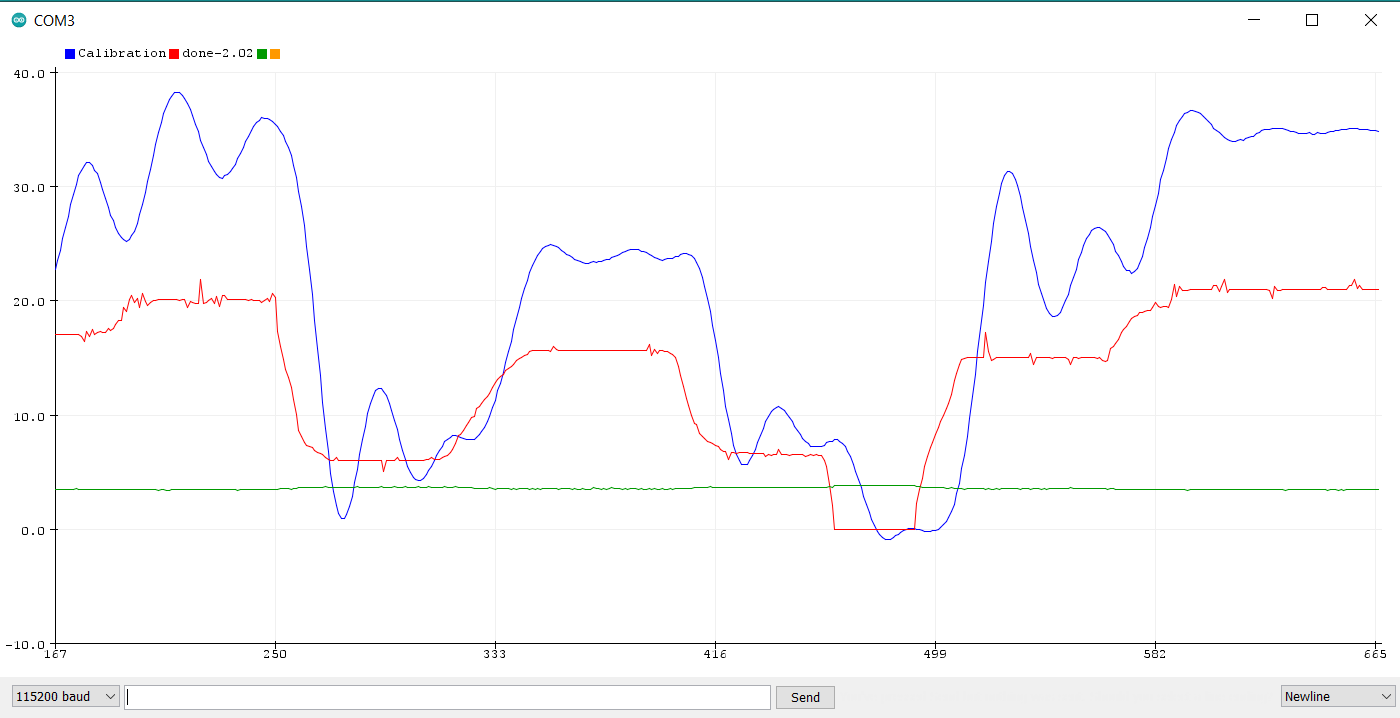
\includegraphics[width=120mm]{obr/VystupOLIDE.png}
	\caption{Výstup z programu AeroShieldOpenLoop.ino.}\label{OBRAZOK 3.1}
\end{figure}

\subsection{MATLAB}

V príklade \verb|AeroShieldOpenLoop.m| si ukážeme výhody a možnosti zobrazovania výstupov, v prostredí MATLAB. Výstupy vieme zobrazovať nielen na sériovom monitore alebo zapisovači, ale máme možnosť tvoriť grafy, tabuľky... a všetky tieto výstupy upravovať a ukladať podľa vlastných predstáv a požiadaviek. 


Na začiatku kódu vymažeme všetky premenné a objekty, pomocou série príkazov \code{Clear all, clear a, clc}. Následne načítame knižnicu AeroShieldu a vykonáme funkciu \verb|AeroShield.begin()|. Nasleduje kalibrácia nulového uhlu kyvadla a zadefinovanie premenných na počítanie času, ako aj premenné na ukladanie hodnôt potenciometra a uhlu kyvadla. 

\begin{lstlisting}[caption={AeroShield open loop inicializacia.},captionpos=b]
% vymazanie premennych a objektov 
clear all;
clear a;
clc 

% nacitanie kniznice AeroShieldu  
AeroShield=AeroShield;
% vytvorenie objektov arduino, as5600
AeroShield.begin();
% kalibracia
startangle= AeroShield.calibration(); 
lastangle=startangle+2048; 

% premenne na pocitanie casu
time = 0;
count = 0;
angle = 0;          % uhol kyvadla
potentiometer = 0;  % hodnota potenciometra
\end{lstlisting}

Ďalej pokračujeme s definovaním vlastností grafu na zobrazovanie hodnôt potenciometra a uhlu kyvadla. Zvolili sme spôsob kontinuálneho vykresľovania grafu, kedy obe strany grafu zobrazujú rozdielne premenné a rozsahy, ktoré sa prispôsobujú veľkosti premenných. Zapisovanie premenných na rôzne strany grafu funguje vďaka príkazom, \verb|yyaxis right| a \verb|yyaxis left|, za ktorými nasleduje samotné vykreslenie grafu pomocou príkazu \verb|plot()|. Volíme si taktiež názvy osí grafu a jeho legendu. Medzi vykresleniami jednotlivých premenných použijeme príkaz \verb|hold on|, ktorý zabezpečí zapísanie premenných do jedného grafu. Na konci kódu je príkaz \verb|tic| ktorý začne počítať prejdený čas, od jeho spustenia. 

\begin{lstlisting}[caption={AeroShield open loop grafy.},captionpos=b]
	yyaxis right                      % set plotting to right axis 
	plotGraph = plot(time,angle,'-r' )      % plotting angle value
	ylabel('Angle (degree)','FontSize',15);      % label settings
	xlabel('Time (s)','FontSize',15);       % label settings
	hold on       % hold on makes sure all of the variables are plotted
	
	yyaxis left                             % Set plotting to left axis
	plotGraph1 = plot(time,potentiometer,'-b') % plotting potentiometer value
	title('Pendulum plot','FontSize',15);      % title settings   
	ylabel('Percent','FontSize',15)            % label settings
	legend('Potentiometer value','Pendulum angle')   % legend for plots
	grid('on');                      % grid for plot 'off' to turn off grid
	
	tic                              % time keeping
\end{lstlisting}

Nasleduje while cyklus ktorý má podmienku ukončenia zatvorenie vykresľovaného grafu tj. v momente kedy zatvoríme graf, podmienka prestane byť splnená a program sa ukončí. V cykle najskôr čítame hodnotu potenciometra pomocou \verb|AeroShield.referenceRead()| a túto hodnotu zapisujeme na akčný člen vďaka príkazu \verb| AeroShield.actuatorWrite()|. Nasleduje čítanie uhlu kyvadla \verb|AeroShield.getRawAngle()|, za ktorím prebehne mapovanie premennej z hodnoty raw na stupne. Premenná \verb|count| slúži na počítanie počtu prejdených cyklov, ako aj na tvorbu usporiadaného radu premenných, a využívame ju aj na vykresľovanie pohyblivej x-ovej osi grafu obr.\ref{OBRAZOK 3.2}. Ľavá stupnica grafu je stacionárna a zobrazuje hodnotu potenciometra, pravá stupnica zobrazuje uhol kyvadla v stupňoch a svoje rozpätie zväčšuje alebo zmenšuje v závislosti na výchylke kyvadla. Na konci programu ešte nájdeme if podmienku, ktorá kontroluje uhol kyvadla. Ak ten nadobudne hodnotu väčšiu ako 110°, proces sa automaticky ukončí a vypíše sa upozornenie. Posledný príkaz \verb|clear AeroShield.arduino| vymaže objekt \verb|arduino| a pripraví MATLAB na spustenie ďalšieho programu. 

\begin{lstlisting}[caption={AeroShield open loop, while cyklus.},captionpos=b]
while ishandle(plotGraph)           % loop will run until plot is closed
	
	pwm = AeroShield.referenceRead();   % read potentiometer value
	AeroShield.actuatorWrite(pwm);      % actuate 
	RAW= AeroShield.getRawAngle();      % read raw angle value
	angle_ = mapped(RAW, startangle, lastangle, 0, 180); % map raw value to degree 
	
	count = count + 1;                              % cycle counter
	time(count) = toc;                              % time keeping
	angle(count) = angle_(1);                       % angle value in time
	percenta= mapped(pwm, 0.0, 5.0, 0.0, 100.0);    % map pwm to percent 
	potentiometer(count) = percenta(1);             % pententiometer value in time
	set(plotGraph,'XData',time,'YData',angle);      % plot first data 
	set(plotGraph1,'XData',time,'YData',potentiometer); % plot second data 
	axis([time(count)-5 time(count) 0 100]);        % "running" x axis settings
	
	if (angle_ > 110)                            % if angle of pendulum bigger than 110degree
	AeroShield.actuatorWrite(0.0);      % stop the motor 
	disp('Angle of pendulum too high. AeroShield is turned off')
	break                               % stop the program
	end
end  

clear AeroShield.arduino;           
\end{lstlisting}

\begin{figure}[!tbh]
	\centering
	\includegraphics[width=\textwidth]{obr/ASOLmat.png}
	\caption{Výstup z programu AeroShieldOpenLoop.m.}\label{OBRAZOK 3.2}
\end{figure}

\newpage
\section{Programy v uzatvorenej slučke, so spätnou väzbou}
\subsection{PID regulácia}

Skôr ako si ukážeme príklady na PID riadenie,musíme si vysvetliť ako takéto riadenie funguje. Základom takéhoto riadenia je získavanie informácii o sledovanej resp. riadenej veličine, za pomoci senzoru a jej porovnávanie s hodnotou žiadanou. Vďaka tomu že získavame informácie o výstupe, ktoré aktívne využívame na riadenie akčného člena, môžeme hovoriť o spätnoväzbovom riadení. Spätnoväzbové riadenie, je teda také riadenie, ktoré ovplyvnuje sústavu na základe aktuálne získaných informácii o stave, v ktorom sa sústava práve nachádza. Pri takomto riadení existuje množstvo algoritmov, ktoré ovládajú správanie sa systému. Medzi tieto algoritmy patrí napríklad: Modelové prediktívne riadenie (MPC), Lineárno-kvadratické riadenie (LQ), Lineárne riadenie s premenlivým parametrom (LPV), Proporcionálno-integračno-derivačné riadenie (PID)...

Bližšie sa ideme baviť o PID regulátore obr.\ref{OBRAZOK 3.3}. Je to typ riadenia, ktoré ovplyvňuje akčné zásahy do sústavy \verb|u(t)|, na základe zaznamenaných výstupných informácii zo sústavy \verb|y(t)|. Veľkosť akčného zásahu \verb|u(t)| vypočítame na základe rozdielu medzi požadovanou hodnotou \verb|w(t)| a hodnotou reálnou \verb|y(t)|. Tento rozdiel označujeme tiež ako regulačná odchýlka \verb|e(t)|. Písmeno $"$t$"$ v zátvorkách predstavuje, časovú závislosť premenných. 

\begin{figure}[!tbh]
	\centering
	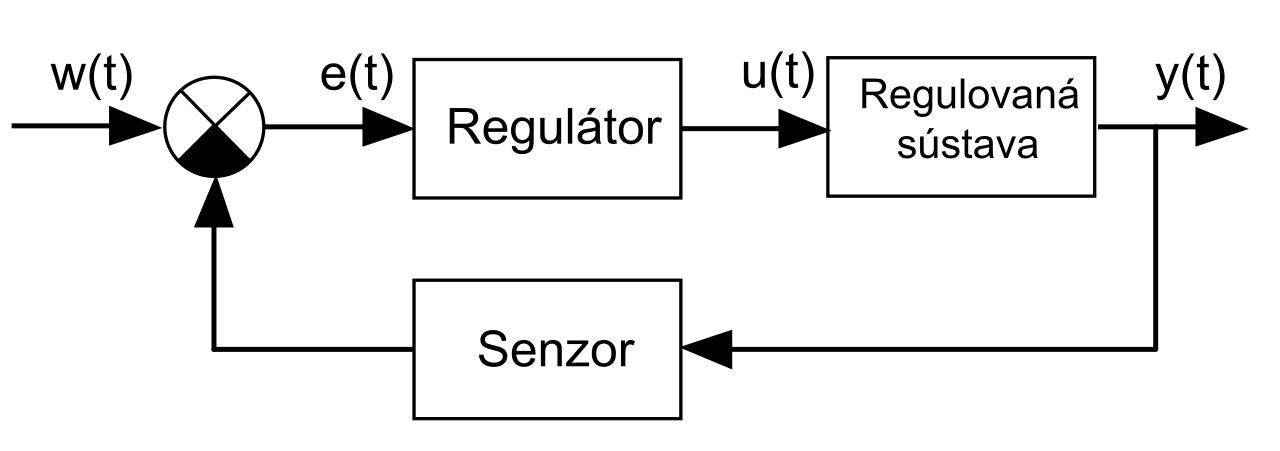
\includegraphics[width=120mm]{obr/pid.jpg}
	\caption{Schéma riadenia PID regulátorom.}\label{OBRAZOK 3.3}
\end{figure}

Skratka PID odzrkadľuje zložky, z ktorých sa regulátor skladá: 

\begin{itemize}
	\item \textbf{P}- označuje tzv. proporcionálnu zložku. Akčný zásah smerujúci do sústavy \verb|u(t)|, je priamo úmerný veľkosti regulačnej odchýlky \verb|e(t)|. K$_p$ predstavuje proporcionálnu konštantu, ktorou násobíme regulačnú odchýlku na získanie požadovaného vstupu rov.\ref{rovnicajedna}. 
	\begin{align}
		\label{rovnicajedna}
		u(t)=K_p e(t)
	\end{align}
	Konštanta K$_p$ je veľmi dôležitou pri nastavovaní parametrov PID regulátora, lebo znižuje trvalú regulačnú odchýlku. Zmenou proporcionálnej zložky vieme taktiež urýchliť, alebo spomaliť nábeh na požadovanú hodnotu. Pre malé hodnoty K$_p$ je nábeh pomalí, a regulačná odchýlka veľká. Pri zvyšovaní hodnoty K$_p$ sa regulačná odchýlka zmenšuje, zrýchľuje sa nábeh, no zároveň narastá nežiadúce kmitanie sústavy. Zvyšovanie hodnoty K$_p$ má svoj limit, za ktorým sa sústava dostáva za hranicu stability a ďalšia regulácia nie je možná. 
	
	\item \textbf{I}- predstavuje integračnú zložku. Integrálny riadiaci člen je priamo úmerný veľkosti ako aj trvaniu chyby. Pokiaľ má regulovaná veličina menšiu hodnotu ako je požadovaná, integrálna časť PID sa zväčšuje. Naopak pokiaľ je hodnota regulovanej veličiny nižšia ako hodnota požadovaná, integrálna časť PID klesá. Tento údaj sa následne vynásobí integračnou konštantou K$_i$ a je pripočítaný ku hodnote akčného zásahu rov.\ref{rovnicadva}. Príliš veľká hodnota K$_i$ má za následok zvyšovanie nežiadúceho kmitania resp. nad a pod regulovania. 
	
	Veľkosť integrálnej zložky PID regulátora teda ovplyvňuje veľkosť regulačnej odchýlky, doba jej trvania ako aj integračná konštanta K$_i$.
	\begin{align}
		\label{rovnicadva}
		u(t)=K_i  \int_{0}^{t} e(\tau)d\tau
	\end{align}

	\item \textbf{D}- reprezentuje derivačnú zložku. Derivačná zložka predpovedá správanie sa systému, pomocou derivácie regulačnej odchýlky v čase. Toto temto zmeny je následne pre násobené derivačnou konštantou K$_d$. Vstup je teda počítaný podľa rov.\ref{rovnicatri}. Derivačná zložka PID regulátora zmierňuje kmitanie systému, zároveň však spomaľuje rýchlosť odozvy na skokovú zmenu. V praxi sa derivačná zložka veľmi nepoužíva a využívaný je P alebo PI regulátor. 
	\begin{align}
		\label{rovnicatri}
		u(t)=K_d  \dfrac{de(t)}{dt}
	\end{align}
\end{itemize}

Pre lepšie chápanie je v tab.\ref{PIDvplyv}\cite{pidcontrol} zhrnutie vplyvu jednotlivých zložiek PID na odozvu systému v uzatvorenej slučke, pri zvyšovaní hodnoty K$_p$, K$_i$ a K$_d$.

\begin{table}[!tbh]
	\begin{tabular}{|c|c|c|c|c|c|}
		\hline
		 & Regulačná odchýlka & Rýchlosť ustálenia & Prekmit & Rýchlosť odozvy & Stabilita \\ \hline
		K$_p$                    & znižuje            & malý vplyv         & zvyšuje      & zvyšuje         & znižuje           \\ \hline
		K$_i$                    & znižuje            & znižuje            & zvyšuje      & zvyšuje         & znižuje           \\ \hline
		K$_d$                    & malý vplyv         & zvyšuje            & znižuje      & znižuje         & zvyšuje           \\ \hline
	\end{tabular}
	\caption{Odozva systému na zmenu konštánt.}
	\label{PIDvplyv}
\end{table}

Spojením jednotlivých samostatných zložiek, získame kompletný vzťah pre PID regulátor rov.\ref{rovnicastr}.
\begin{align}
	\label{rovnicastr}
	u(t)=K_p e(t) + K_i  \int_{0}^{t} e(\tau)d\tau + K_d  \dfrac{de(t)}{dt}
\end{align}

\begin{align}
	\label{rovnicapat}
	u(t)=K_p \left(e(t) + \dfrac{1}{T_i}  \int_{0}^{t} e(\tau)d\tau + T_d  \dfrac{de(t)}{dt}\right)
\end{align}
Rovnica \ref{rovnicastr} predstavuje jeden z možných tvarov zápisu vzťahu pre PID regulátor. V praxi sa často využíva tvar rov.\ref{rovnicapat}, z dôvodu lepšej interpretácie parametrov ktoré rovnicu tvoria. T$_i$ predstavuje integračnú a T$_d$ derivačnú časovú konštantu, pričom ich vzťah s konštantami K$_i$ a K$_d$ je v tvare T$_i$ = (K$_p$/K$_i$) a T$_d$ = (K$_d$/K$_p$). Jednotlivé zložky v zátvorke tvoria novú a samostatnú regulačnú odchýlku, ktorá je ešte násobená konštantou K$_p$. Derivačná zložka predpovedá hodnotu regulačnej odchýlky T$_d$ sekúnd(vzoriek) do budúcnosti a integračná zložka sa snaží korigovať súčet hodnoty regulačných odchýlok do T$_i$ sekúnd(vzoriek)\cite{pidcontrol}.

Spomenuté vzťahy PID regulátorov fungujú pri spojitých procesoch. Avšak pri implementácii PID pomocou číslicových regulátorov, musíme rovnicu transformovať do jej diskrétnej podoby rov.\ref{diskretna}.

\begin{align}
	\label{diskretna}
	u(kT)=K_p \left(e(kT) + \dfrac{T}{T_i} \sum_{i=0}^{k}  e(iT) + \dfrac{T_d}{T} \left[e(kT)-e \left[(k - 1)T\right] \right] \right)
\end{align}

Diskrétna forma PID regulátora je využívaná z toho dôvodu že Arduino resp. počítače nie sú schopné nepretržito zaznamenávať merané hodnoty. Dáta sú preto spracovávané v diskrétnych okamihoch kT, ktorým hovoríme vzorky. Proces získavania takýchto vzoriek v istej pravidelnom frekvencii, nazývame vzorkovanie. Vzorkovanie môže mať rýchlosť niekoľko minút, pri pomali sa meniacich systémoch, až po mikrosekundy, pri veľmi rýchlych systémoch. Rovnicu v tvare \ref{diskretna} využíva na implementáciu PID regulátora knižnica AutomationShield a teda je aj súčasťou didaktických príkladov pre AeroShield. 

\section{Príklady riadenia pomocou PID regulátora}
\subsection{Arduino IDE}
\label{Arduino IDE PID}

V tomto príklade využívame na riadenie PID regulátora, vopred pripravenú knižnicu \verb|PIDAbs|, ktorá je volaná z knižnice \verb|AeroShield|. Za účelom vzorkovania, využívame knižnicu \verb|Sampling|, ktorú načítame do príkladu príkazom \code{#include <Sampling.h>}. Pri voľbe referenčnej trajektórie máme na výber z dvoch možností. Prvou je voľba manuálnej trajektórie, ktorej referenčnú hodnotu nastavujeme pomocou potenciometra na shielde. Druhou voľbou je automatická trajektória, ktorá má vopred naprogramované referenčné hodnoty. Voľbu trajektórie meníme zmenou hodnoty premennej \verb|MANUAL| z 0 na 1 v príkaze \code{#define MANUAL 0}. Parametre regulátora K$_p$, T$_i$ a T$_d$ slúžia ako symbolické parametre, pre lepší prehľad. Ich hodnotu zapisujeme do PID knižnice pomocou metódy \code{PIDAbs.setKp(KP)}. Vzorkovacia perióda \verb|Ts| je nastavená na hodnotu troch milisekúnd. Perióda vzorkovania je priradená riadiacemu algoritmu PID, ako aj knižnici na vzorkovanie. 

\begin{lstlisting}[caption={Načítanie knižníc a premenných do programu.},captionpos=b]
#define KP 1.7          // PID Kp konstanta
#define TI 3.8          // PID Ti konstanta
#define TD 0.25         // PID Td konstanta

float startAngle=0;     //  Premenna pre nulovy uhol kyvadla
float lastAngle=0;      //  Premenna pre mapovanie uhlu kyvadla
float pendulumAngle;    //  Realna hodnota uhlu kyvadla

unsigned long Ts = 3;   // Vzorkovacia perioda 
unsigned long k = 0;    // Index vzorky 
bool nextStep = false;  // Povolenie kroku vzorky 
bool realTimeViolation = false;     // Premenna pri poruseni vzorkovania

int i=i;                // Index referencnej hodnoty 
int T=1000;             // Dlzka sekcie dana poctom vzoriek 
float R[]={45.0,23.0,75.0,32.0,58.0,10.0,35.0,
	19.0,9.0,43.0,23.0,65.0,15.0,80.0};  // Referencna trajektoria kyvadla
float r = 0.0;          // Referencia (Uhol ktory chceme dosiahnut)
float y = 0.0;          // Vystup (Realny uhol kyvadla)
float u = 0.0;          // Vstup (Vykon motora)
\end{lstlisting}

V organizačnej funkcii setup sa nastaví rýchlosť sériovej komunikácie, spolu s inicializáciou a kalibráciou AeroShieldu. Zároveň sa nastavia hodnoty PID 
regulátora, ako aj rýchlosť vzorkovania.  

\begin{lstlisting}[caption={Organzačná funkcia setup.},captionpos=b]
void setup() {   
	Serial.begin(250000);      //  Zaciatok seriovej komunikacie
	AeroShield.begin();   //  Inicializacia 
	startAngle = AeroShield.calibration(AeroShield.getRawAngle());        // Kalibracia
	lastAngle=startAngle+1024;       // Vypocet uhlu pre mapovanie 
	Sampling.period(Ts*1000);              // Vzorkovacia perioda 
	PIDAbs.setKp(KP);                      // Nastavenie Kp
	PIDAbs.setTi(TI);                      // Nastavenie Ti
	PIDAbs.setTd(TD);                      // Nastavenie Td
	PIDAbs.setTs(Sampling.samplingPeriod); // Vzorkovacia perioda
	Sampling.interrupt(stepEnable);  				   // Nasatavenie nazvu funkcie stepEnable, v kniznici sampling 
}
\end{lstlisting}

Funkcia \verb|stepEnable()| je volaná z knižnice sampling, v intervale zadanom na začiatku programu, ako vzorkovacia perióda. Slúži na kontrolu postupnosti vzoriek a povolenie spustenia nasledujúcej vzorky. Táto funkcia je volaná vždy len na začiatku jednotlivých vzoriek. Pokiaľ je teda v trvaní jednej vzorky spustená viacero krát, vieme povedať že nastala chyba vzorkovania. Pri takejto chybe sa vypne motor a pomocou príkazu \code{while(1)}, je ukončené vykonávanie programu. 

Pokiaľ nedošlo ku chybe vzorkovania, funkcia povolí vykonanie nasledujúcej vzorky, zmenou hodnoty premennej \verb|nextStep|, na hodnotu $"$true$"$ teda 1. 

\begin{lstlisting}[caption={Funkcia stepEnable().},captionpos=b]
void stepEnable() {                          
	if(nextStep == true) {        // Pokial predosla vzorka stale trva
		realTimeViolation = true; // Nastala chyba vzorkovania
		Serial.println("Real-time samples violated."); 			// Vypis chybovu hlasku
		analogWrite(5,0);         // Vypni motor 
		while(1);                 // Ukonci vykonavanie programu
	}
	nextStep = true;              // Povol nasledujucu vzorku
}
\end{lstlisting}

V organizačnej funkcii \code{loop()}, je ako prvá, kontrolovaná podmienka \code{if(pendulumAngle>120)}. Táto kontrola slúži ako ochranný mechanizmus, pred pretočením kyvadla o príliš veľký uhol. Ďalej je v rámci vzorkovania volaná funkcia \verb|step()|. V if podmienke je testovaná premenná nextStep. Pokiaľ táto premenná nadobudne hodnotu "true", teda 1, podmienka sa splní a vykoná sa funkcia \verb|step()|, za ktorou sa premennej nextStep priradí hodnota "false", teda 0.

\begin{lstlisting}[caption={Organzačná funkcia loop.},captionpos=b]
void loop() {
	if(pendulumAngle>120){		// Bezpecnostna podmienka kyvadla 
		AeroShield.actuatorWrite(0); // Pokial je uhol vacsi ako 120
		while(1);		// stupnov, motor sa vypne
	} 
	if (nextStep) {         // Pokial nextStep == 1
		step();             // Spusti funciu step()
		nextStep = false;   // Vynuluj premennu 
	}
}
\end{lstlisting}

Funkcia \verb|step()| vykonáva samotné meranie, ovládanie a výpočty potrebné pri riadení systému pomocou PID regulátora. Na začiatku funkcie sa zvolí buď manuálna, alebo automatická trajektória. Pri automatickej dráhe je dôležité, vedieť kedy bol dosiahnutý koniec pred programovanej trajektórie. Táto kontrola je vykonávaná pomocou porovnávania veľkostí premennej \verb|i|, ktorá zaznamenáva počet vykonaných sekcií trajektórie, oproti veľkosti pola \verb|R[]|, v ktorom sú zapísané hodnoty jednotlivých sekcií. Príkaz \code{sizeof(R)/sizeof(R[0])}, vráti počet prvkov pola \verb|R[]|. Zároveň sa kontroluje dĺžka chodu sekcie. Pokiaľ výraz \verb|k % (T*i)|, dosiahne hodnotu 0, nastaví sa ako trajektória nasledujúca sekcia. 

Následne je mapovaný uhol kyvadla na percentuálnu hodnotu od 0\% do 100\%, ktorá je uložená ako premenná \verb|y|. Veľkosť regulačnej odchýlky, obmedzenie integračného nasýtenia\footnote[9]{K nasýteniu integračnej zložky dochádza, v prípade že akčný člen nie je schopný dosiahnuť požadovanú referenčnú
	hodnotu. V takom prípade začne hodnota integračná zložka nekontrolovateľne stúpať.}(angl. anti-windup), ako aj hodnotu saturácie systému\footnote[10]{Keď sa hodnota spätnoväzbového riadiaceho systému dostane do oblasti nasýtenia ktorejkoľvek z jeho zložiek, zmena vstupu nasýtenej zložky nespôsobí žiadnu zmenu na jej výstupe. Zosilnenie vtedy dosahuje nulové hodnoty.}, zadávame do algoritmu na výpočet akčného zásahu v tvare \verb|PIDAbs.compute(r-y,minSaturacia,maxSaturacia|
\verb|,antiWindupMin,antiWindupMax);|. 


\begin{lstlisting}[caption={Funkcia step().},captionpos=b]
void step() {            
	#if MANUAL    // Pokial je zvolena manualna trajektoria 
	r = AeroShield.referenceRead();     // Referencna hodnota z potenciometra
	#else         
	if(i>(sizeof(R)/sizeof(R[0]))) {    // Pokial automaticka trajektoria skoncila
		analogWrite(5,0);           // Vypni motor
		while(1);                   // Zastav program
	} else if (k % (T*i) == 0) {  // Pokial je dosiahnuty koniec       sekcie trajektorie
		r = R[i];        // Postup na dalsiu sekciu
		i++;             // Pripocitaj postup o jednu sekciu 
	}
	#endif
	
    y= AutomationShield.mapFloat(AeroShield.getRawAngle(),startangle,lastangle,0.00,100.00);
	// Mapovanie uhlu kyvadla na percenta 
	u = PIDAbs.compute(r-y,0,100,0,100);  // Vypocet PID 
	AeroShield.actuatorWrite(u);          // Aktuator
	
	Serial.print(r);           // Referencna hodnota 
	Serial.print(", ");
	Serial.print(y);           // Vystup 
	Serial.print(", ");
	Serial.println(u);         // Akcny zasah 
	k++;                       // Pocitadlo vzoriek 
}
\end{lstlisting}

\subsubsection{Výstupy}

Všetky výstupy z API Arduino IDE, boli zaznamenávané programom CoolTerm a následne vykreslené do grafov v prostredí MATLAB. 

Na obr.\ref{OBRAZOK 2.5.1}, vidíme reakciu systému na skokovú zmenu z nulovej referenčnej hodnoty na hodnotu maximálnu, teda 100\%. Pomocou sledovania odozvy systému vieme lepšie nastaviť parametre PID regulátora. Systém nadobudne 1\% regulačnú odchýlku v priebehu 500 vzoriek, čo znamená čas približne jeden a pol sekundy. 

\begin{figure}[!tbh]
	\centering
	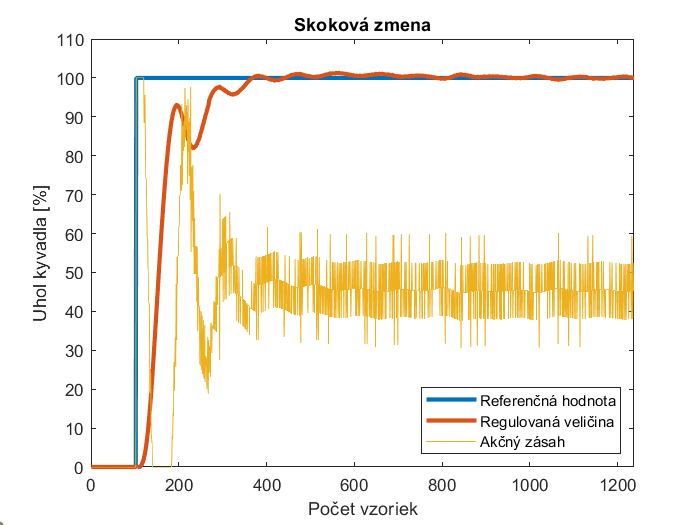
\includegraphics[width=\textwidth]{obr/SkokovaZmena.png}
	\caption{Reakcia systému na jednotkový skok.}\label{OBRAZOK 2.5.1}
\end{figure}

Manuálna trajektória obr.\ref{OBRAZOK 2.5.3}, má oproti automatickej trajektórii obr.\ref{OBRAZOK 2.5.2}, väčšie rozdiely v hodnote akčného zásahu. Je to spôsobené kontinuálnou zmenou referenčnej hodnoty, ako aj miernym šumom signálu z potenciometra. V rámci obr.\ref{OBRAZOK 2.5.3} si ešte môžeme všimnúť časť medzi vzorkami 5000-6000, ktorá je priblížená na obr.\ref{OBRAZOK 2.5.4}. Jedná sa o manuálne zavedenie výchylky, pomocou buchnutia do kyvadla. Systém na takúto zmenu reaguje zmenou akčného zásahu a regulačnú odchýlky menšiu ako 2\%, nadobúda v priebehu jednej sekundy. 

\begin{figure}[!tbh]
	\centering
	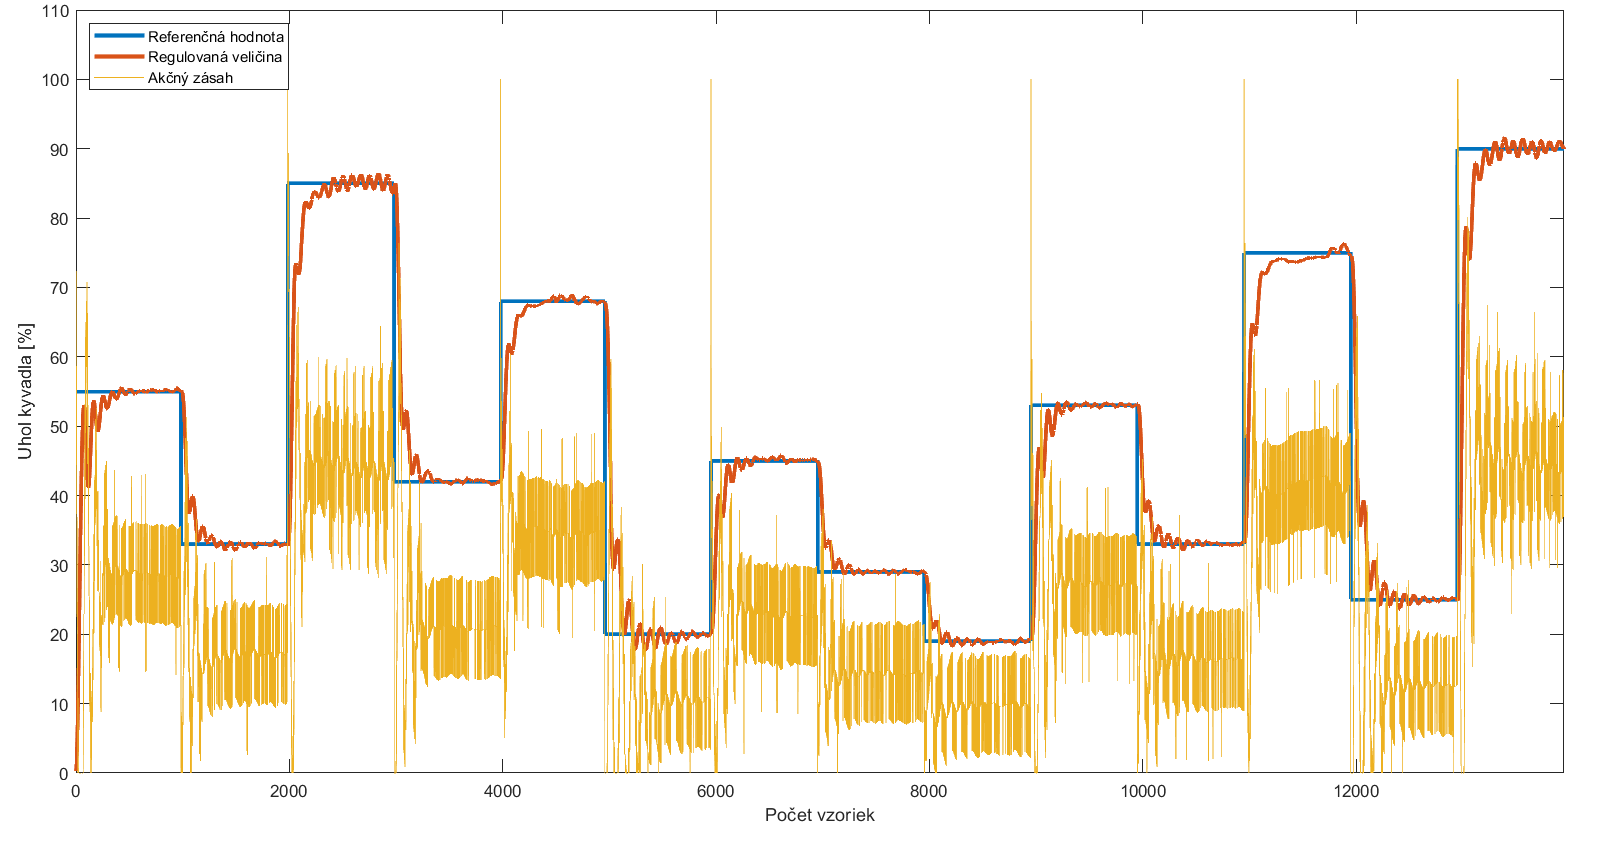
\includegraphics[width=150mm]{obr/Auto3.png}
	\caption{Automatická trajektória.}\label{OBRAZOK 2.5.2}
\end{figure}
\begin{figure}[!tbh]
	\centering
	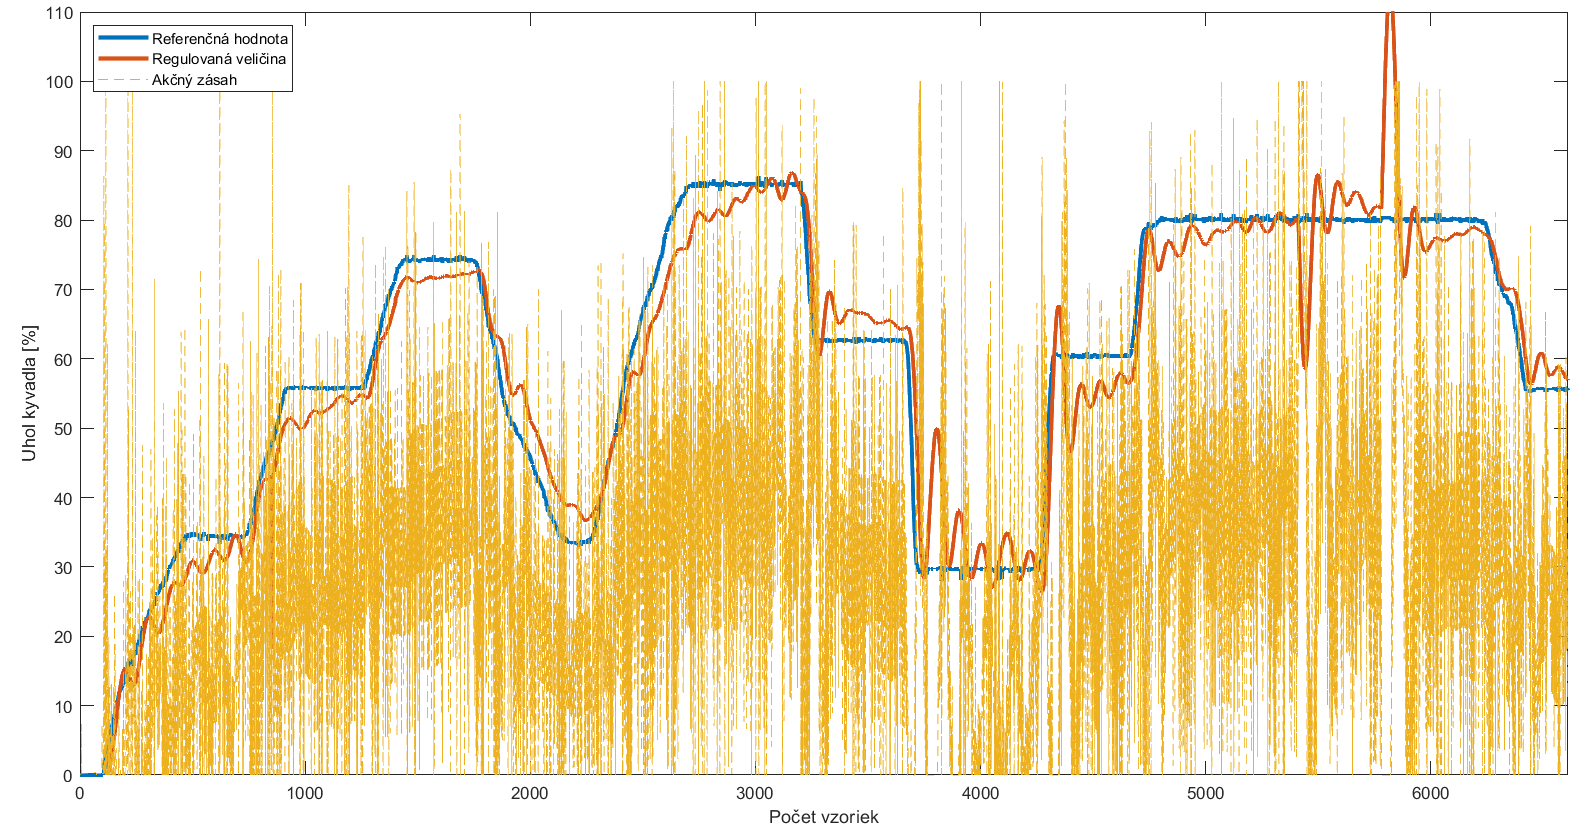
\includegraphics[width=150mm]{obr/potentio.png}
	\caption{Manuálna trajektória.}\label{OBRAZOK 2.5.3}
\end{figure}

\begin{figure}[!tbh]
	\centering
	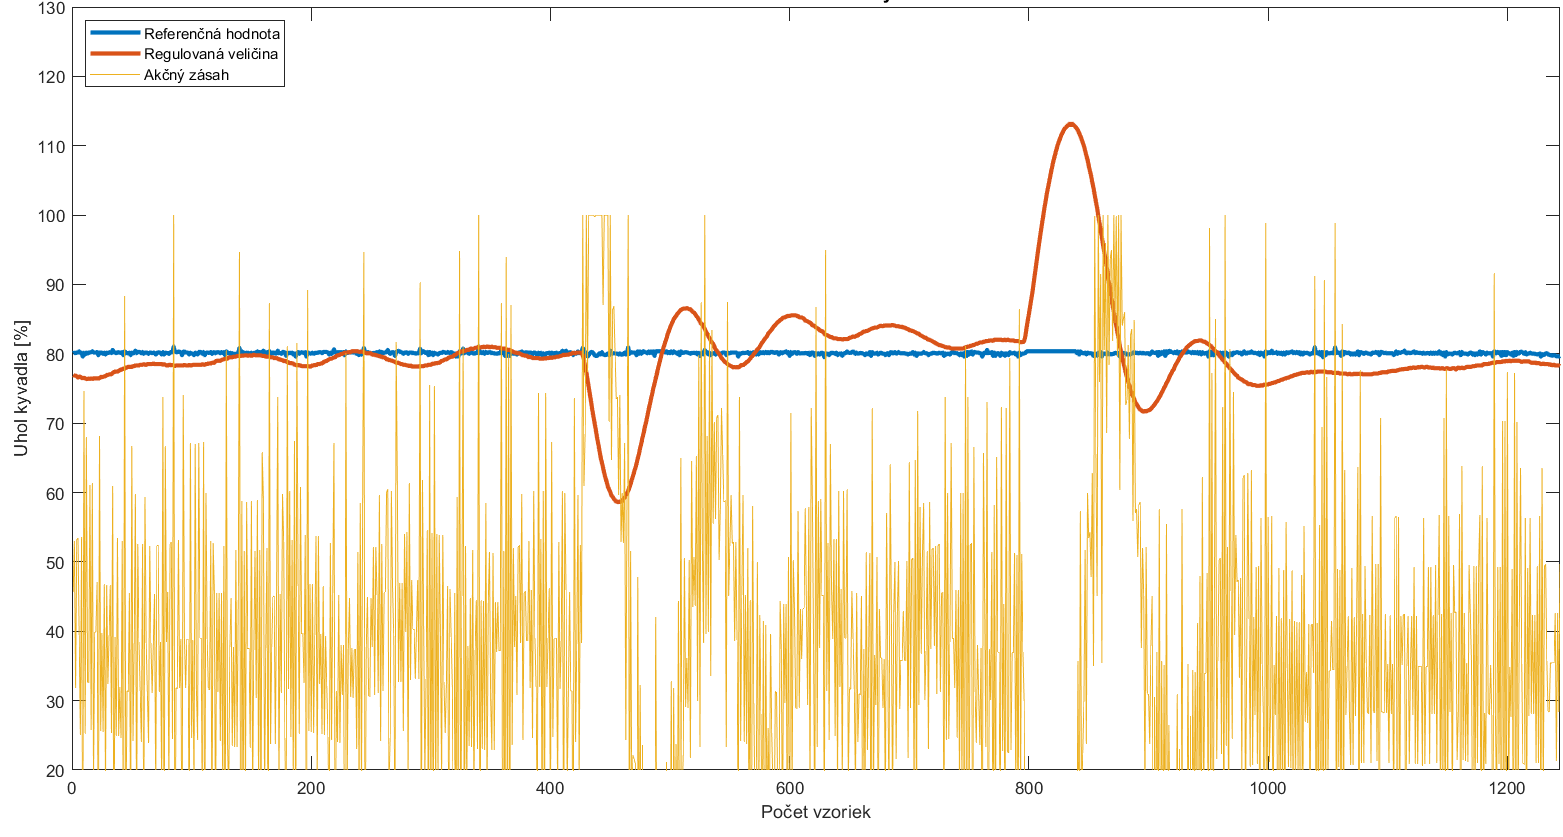
\includegraphics[width=\textwidth]{obr/BuchnutieKyvadla.png}
	\caption{Manuálne zavedenie výchylky .}\label{OBRAZOK 2.5.4}
\end{figure}


\subsection{MATLAB}
\label{MATLABPID}

Príklad na ukážku fungovania PID regulátora bol taktiež vytvorený v prostredí MATLAB a simulink. Princíp fungovania PID regulátora je rovnaký ako pri Arduino IDE, avšak mení sa spôsob vzorkovania a nastavovania parametrov PID. V prípade MATLABU využívame, na výpočet akčného zásahu, knižnicu PID.m, ktorá bola taktiež vytvorená v rámci programu AutomationShield. Na nastavenie parametrov PID slúži príkaz \code{PID.setParameters(Kp, Ti, Td, Ts)}, Ts udáva vzorkovaciu periódu. 

Na vzorkovanie využívame funkcie \verb|TIC a TOC |, ktoré merajú prejdený čas. Funkcia TIC zaznamenáva aktuálny čas a funkcia TOC používa zaznamenanú hodnotu na výpočet uplynulého času. Ak je splnená podmienka \code{if (toc>=Ts*k)}, povolí sa posun na nasledujúcu vzorku, pričom premenná \verb*|k|, udáva počet vykonaných vzoriek. Dáta sú postupne zapisované do poľa \code{ PIDresponse(k,:)=[r y u]}, a toto pole je vykresľované pomocou funkcie \code{plotLive(PIDresponse(k,:))}. Na konci sú všetky dáta uložené, a teda sú prístupné aj po ukončený programu. Kompletný zdrojový kód sa nachádza v prílohe na strane \pageref{AeroShieldPID.m}.

Regulácia PID v prostredí MATLAB potrebuje pre svoje fungovanie pomerne vysoký výpočtový výkon. Z tohoto dôvodu je perióda vzorkovania, oproti Arduino IDE, rádovo nižšia a dosahuje hodnoty maximálne piatich vzoriek za sekundu tj. Ts=0.2s. Takáto rýchlosť vzorkovania je hraničná a teda pri pomalšom vzorkovaní systém nedosahuje ideálne vlastnosti. Výpočtová náročnosť sa dá znížiť, zamedzením vykresľovania grafu, alebo odstránením možnosti ukladania zaznamenaných dát. 

\newpage
\subsubsection{Výstupy}

Všetky výstupy z príkladu \ref{MATLABPID}, majú priamu funkciu vykresľovania grafov spolu s legendou výstupov. Tieto grafy majú taktiež definovaný rozsah zobrazovaných hodnôt na oboch osiach, ako aj pomenovania týchto osí. Na obr.\ref{OBRAZOK 2.6.1} vidíme reakciu systému na jednotkový skok. Obrázok \ref{OBRAZOK 2.6.2} zobrazuje automatickú trajektóriu referenčnej hodnoty a obr.\ref{OBRAZOK 2.6.3} trajektóriu manuálnu. 

\begin{figure}[!tbh]
	\centering
	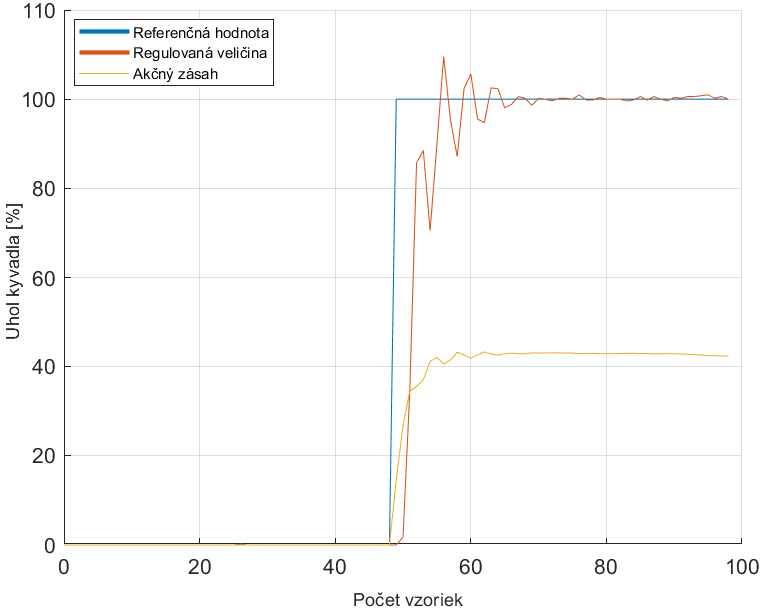
\includegraphics[width=140mm]{obr/jednotkovyskoskMAt.png}
	\caption{Reakcia systému na jednotkový skok.}\label{OBRAZOK 2.6.1}
\end{figure}

Pri manuálnej trajektórii bola trikrát vnesená veľká regulačná odchýlka a to pomocou úderu do kyvadla. Ako je vidieť z grafu \ref{OBRAZOK 2.6.3}, ustálenie systému prebieha oveľa pomalšie ako v príklade \ref{Arduino IDE PID}. Oscilácia je pomerne vysoká a pretrváva po dobu cca 35 vzoriek, čo predstavuje približne 7 sekúnd. Táto skutočnosť je spôsobená pomalšou reakciou PID regulátora, na veľkú regulačnú odchýlku. Dlhší čas potrebný na ustálenie kyvadla je spôsobený pomalším vzorkovaním, ako aj nie ideálne nastavenými hodnotami PID regulátora.  
\vspace{6cm}

\begin{figure}[!tbh]
	\centering
	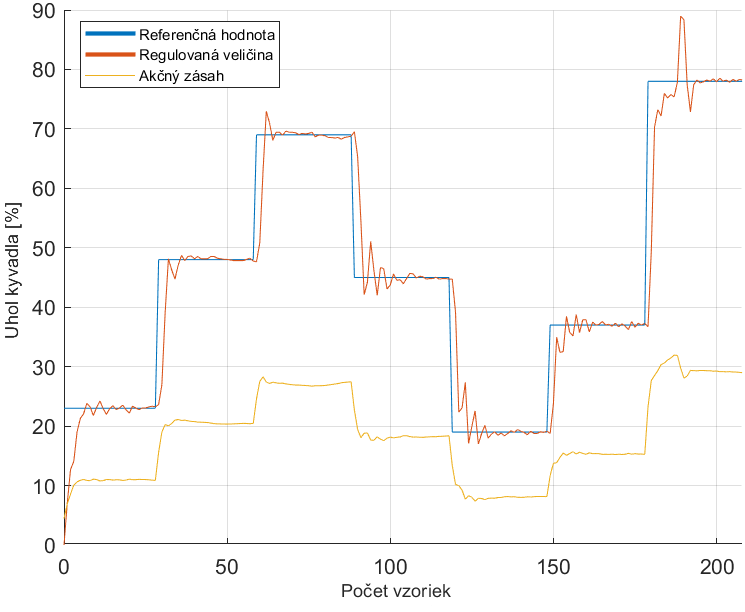
\includegraphics[width=125mm]{obr/PIDautomaMat.png}
	\caption{Automatická trajektória.}\label{OBRAZOK 2.6.2}
	
	\centering
	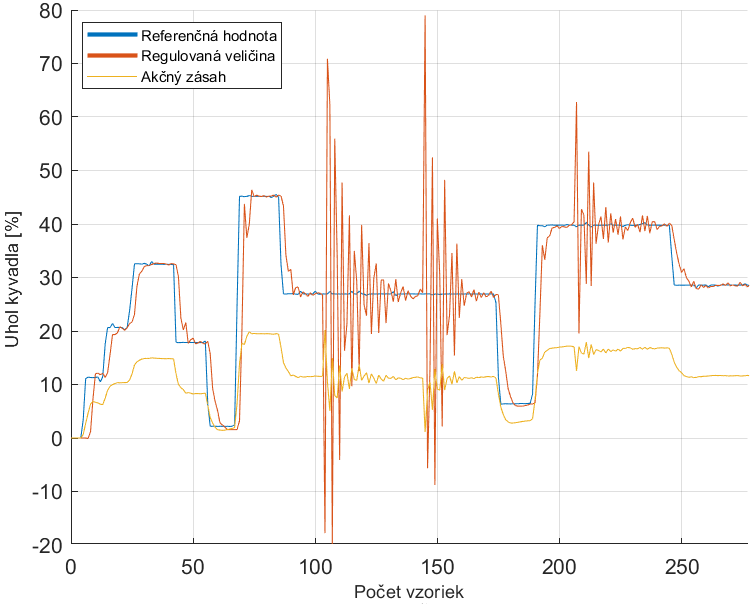
\includegraphics[width=125mm]{obr/pidmanualbuch.png}
	\caption{Manuálna trajektória.}\label{OBRAZOK 2.6.3}
\end{figure}


\subsection{Simulink}

Simulink, narozdiel od MATLABU alebo Arduino IDE, využíva grafické programátorské prostredie, ktoré je založené na prepájaní funkčných blokov, vyberaných z prostredia knižnice. Pre prácu s Arduinom v rámci Simulinku existuje knižnica \textit{Simulink Support Package for Arduino Hardware}, ako aj knižnica AeroLibrary obr.\ref{OBRAZOK 2.6.4}, ktorú využívame priamo pre funkcie AeroShieldu. V knižnici AeroLibrary sa nachádzajú tieto hlavné funkcie: 
\begin{itemize}
\item Reference read- čítanie referenčnej hodnoty 
\item Actuator write- ovládanie akčného členu 
\item Angle read- meranie výstupu 
\item AeroShield- súhrn blokov na zapisovanie akčného zásahu ako aj meranie regulovanej veličiny
\end{itemize}

\begin{figure}[!tbh]
	\centering
	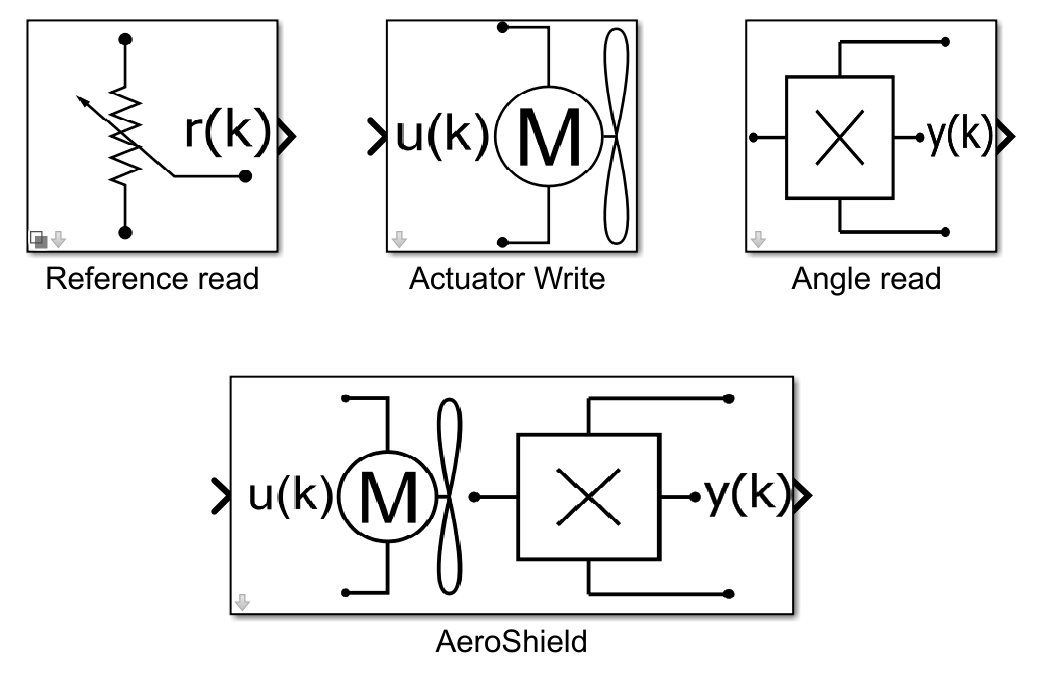
\includegraphics[width=125mm]{obr/AeroLib.png}
	\caption{Knižnica AeroLibrary.}\label{OBRAZOK 2.6.4}
\end{figure}